\documentclass[acmtog]{acmart}
\usepackage{graphicx}
\usepackage{subfigure}
\usepackage{natbib}
\usepackage{listings}
\usepackage{bm}
\usepackage{amsmath}

\definecolor{blve}{rgb}{0.3372549 , 0.61176471, 0.83921569}
\definecolor{gr33n}{rgb}{0.29019608, 0.7372549, 0.64705882}
\makeatletter
\lst@InstallKeywords k{class}{classstyle}\slshape{classstyle}{}ld
\makeatother
\lstset{language=C++,
	basicstyle=\ttfamily,
	keywordstyle=\color{blve}\ttfamily,
	stringstyle=\color{red}\ttfamily,
	commentstyle=\color{magenta}\ttfamily,
	morecomment=[l][\color{magenta}]{\#},
	classstyle = \bfseries\color{gr33n}, 
	tabsize=2
}
\lstset{basicstyle=\ttfamily}

% Title portion
\title{Assignment 5:\\ {Animation with Cloth Simulation}} 

\author{Name:\quad Haoyuan Tian  \\ student number:\ 2020533013
\\email:\quad tianhy@shanghaitech.edu.cn}

% Document starts
\begin{document}
\maketitle

\vspace*{2 ex}

\section{Introduction}
Works that have been done are as follows.
\begin{itemize}
	\item Task1 Force computation with Hooke's law.
	\item Task2 Structural, shear, and bending springs.
	\item Task3 Fix the location of two mesh points to stop the cloth falling down.
	\item Task4 Real-time and stable animation.
	\item Bonus1 Apply external forces to the cloth to simulate the behavior of wind.
	\item Bonus2 Add a sphere or cube obstacle to simulate a piece of cloth falling on a sphere or a cube with collision handling.
	\item Bonus3 Drag a mesh point to move the cloth with mouse in real-time.
\end{itemize}
\section{Implementation Details}

\subsection{Task1 Force computation with Hooke's law}
Most of the code that I need to implement in this assignmnet locates in the file cloth.cpp. The first task, just as the sequence of the codes shown in cloth.cpp, is to implement Hooke's law on two masses to compute the force on one of them.\\
For two masses on the same cloth, named P and Q, we have to calculate the force that Q exerts on P. Use the position of P to substract the position of Q, then we can get the vertex PQ, where the Hooke force is along this direction.\\
Use the following formular to compute the Hooke force, $$F = k(L_0-||p-q||)\frac{p-q}{||p-q||},$$
where L is the zero-force distance of the system, and k is the stiffness.

\subsection{Task2 Structural, shear, and bending springs.}
Then goes into the function ComputeSpringForce().\\
Ensuring the accepted point is right on the cloth, and it is not a fixed point is necessary. Then we have to consider three types of springs of each mass, that is structural, shear and bending springs, each of four other masses that should influence the mass under consideration.\\
As for structural springs, we have to consider the mass affected by its left, right, up and down masses by Hooke force, and we should set the parametre by the distance of the mass, which should be obtained by scale of the object.\\
As for shear springs, we have to consider other 4 masses in the sudoku of the mass under consideration. And for bending springs, we have to consider four farther masses from the mass under consideration.\\
Add them up since all of the 12 masses integrally exert force on the centre mass.

\subsection{Task3 Fix the location of two mesh points to stop the cloth falling down}
Use the interface SetMassFixedOrNot() to set the fix status of a mass, when calculating the physical properties of the mass, such as its acceleration, velocity and its position, we take special consideration on masses that is fixed.\\
As for computing acceleration, we can simply set the acceleration of fixed points to zero. And for computing velocity it should also be zero. And the position of the fixed points remains.
\subsection{Task4 Real-time and stable animation}
All parts of real time animation have been implemented except updating physical status of the cloth, considering each mass on the cloth.\\
Remember that we do all the above calculations in world coordinate, and we should resume it back to local coordinate after those operations.\\
The (static) result is as follows:
\begin{figure}[h]
	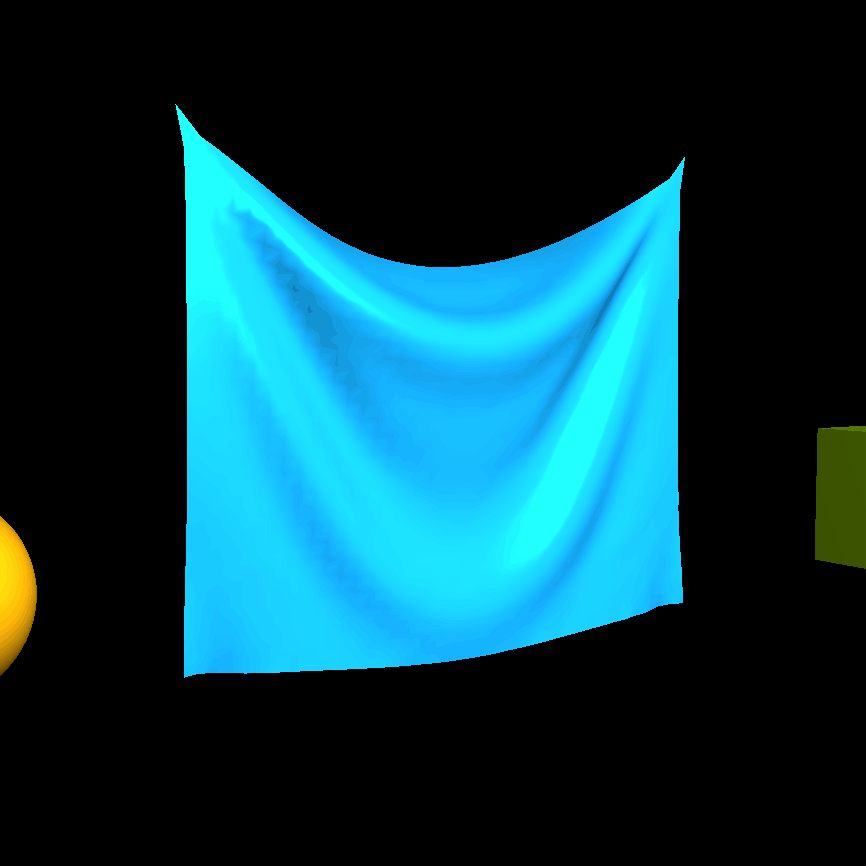
\includegraphics[width=6cm,height=6cm]{must.png}
	\caption{must part}
\end{figure}

\subsection{Bonus1 Apply external forces to the cloth to simulate the behavior of wind}
In the above part, we calculate the force of each mass by adding up total Hooke force exerted on it and (minus) the damping force. Here in this part, we have to add one more force to it, which is exerted by a constant speed wind.\\
I make the speed of the wind a constant, and we can easily get the velocity difference between the wind and each mass, when calculating the force, the array world\_velocity keeps all velovity of masses of last frame.\\
The real influential part of the wind should be the difference velocity times $\cos{\theta}$, where $\theta$ is the angle of the mass' normal and the difference velocity direction. Then return the fluidforce as $$F=kv,$$ in the direction if the mass' normal.\\
Add the fluid force to the total force of each mass, then we get the result (in a flash):
\begin{figure}[h]
	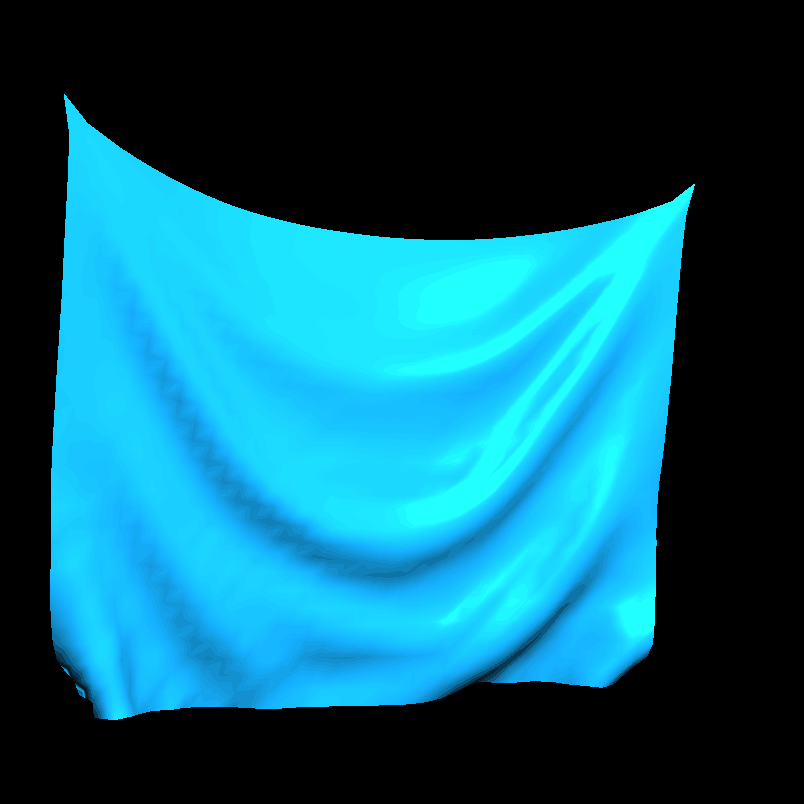
\includegraphics[width=6cm,height=6cm]{wind1.png}
	\caption{fluid force added}
\end{figure}
\subsection{Bonus2 Add a sphere or cube obstacle to simulate a piece of cloth falling on a sphere or a cube with collision handling}
The collision handling can be achieved by considering the intersect situation of a mass and a sphere, here we take sphere as an example. We may consider the intersect situation simply as $||P-shpereCentre||\leq sphereRadius$. However, the sphere is not perfect but is triangular mesh, so we have to take some tolerance of the intersect, otherwise it would perform badly. So the ineaquation I implemented is $$||P-shpereCentre||\leq sphereRadius+INTERSECT\_TOLERANCE.$$
When the cloth intersects with the sphere, we should set the velocity of particular mass to zero, and as well as its acceleration. As for the position, if the position remains, the result would looks like the cloth stick on the sphere, since it would always be judged as intersected. Here I make the mass a little bit outer, along the direction of the mass' normal. Then it should always be judged whether it intersects the sphere in the next frame, and it is more physically resonable that the cloth is covering the sphere, that still has some air between both of them, but not coincide with the sphere.
The result looks like that:
\begin{figure}[h]
	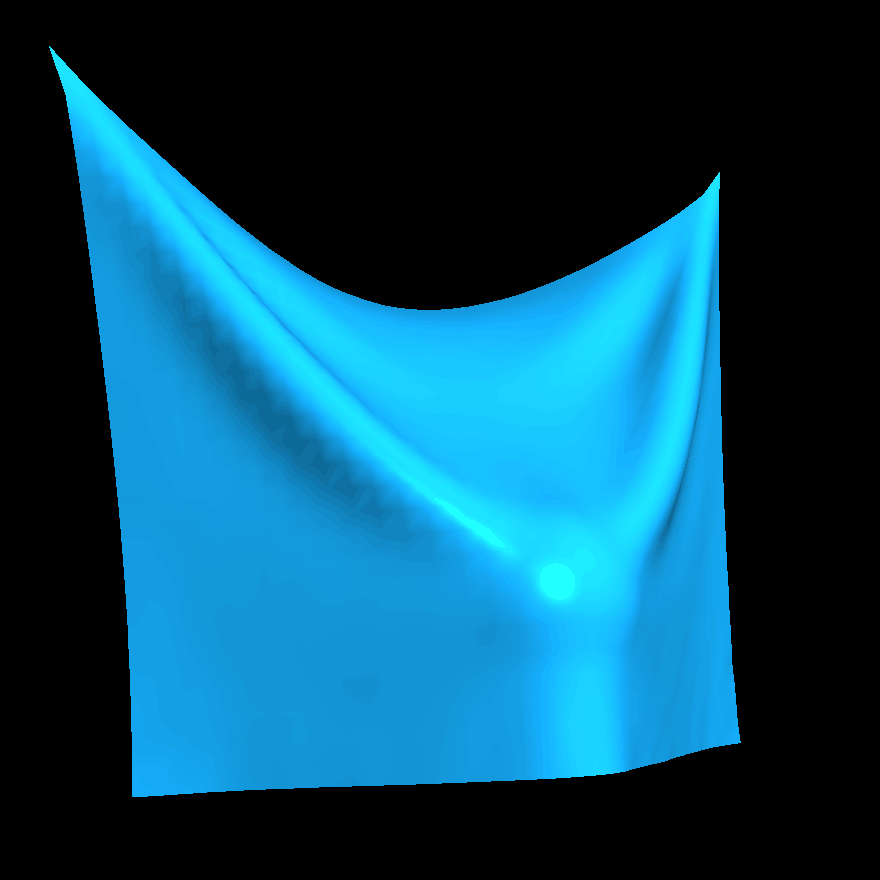
\includegraphics[width=6cm,height=6cm]{sphereObstacle1.png}
	\caption{smaller sphere}
\end{figure}
and making the sphere lager:
\begin{figure}[h]
	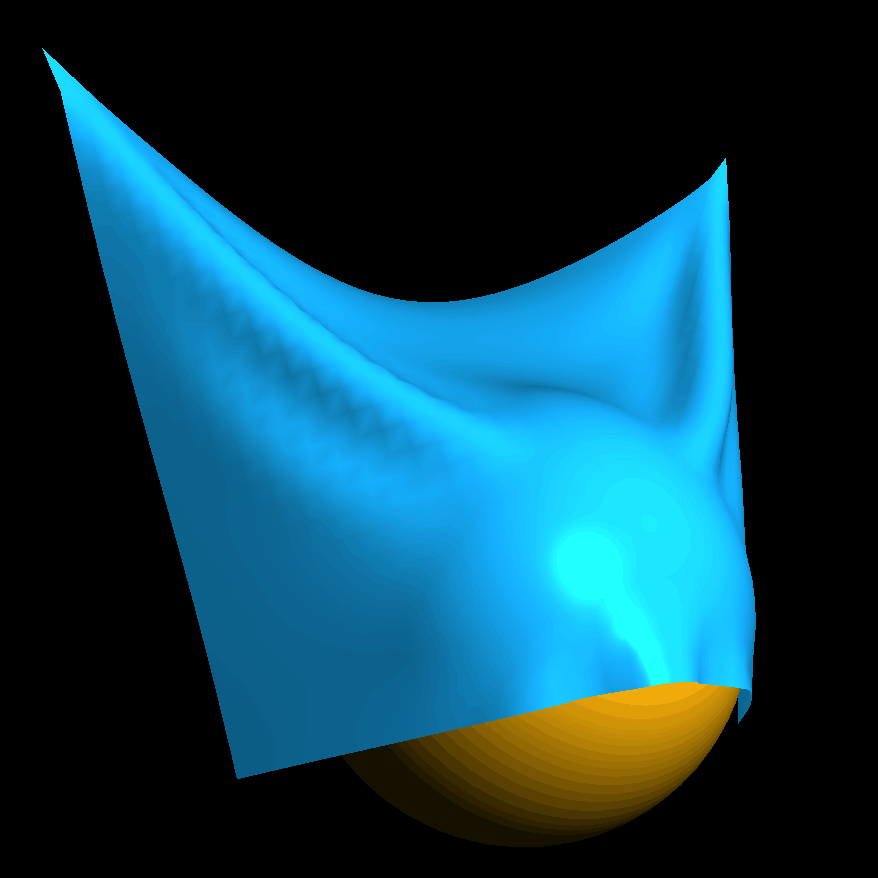
\includegraphics[width=6cm,height=6cm]{sphereObstacle2.png}
	\caption{larger sphere}
\end{figure}
Then taking the fluid implemented in last task into consideration,
\begin{figure}[h]
	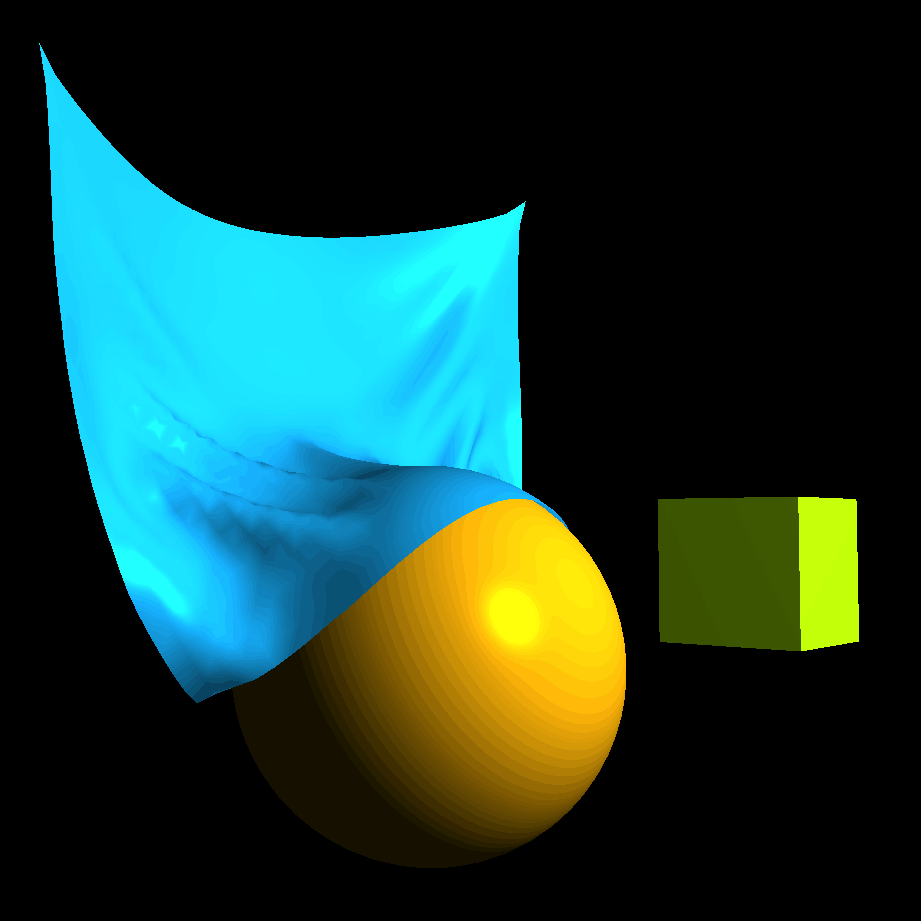
\includegraphics[width=6cm,height=6cm]{wind2.png}
	\caption{larger sphere with fluid force}
\end{figure}
You can see that the fluid can blow the cloth off from the sphere surface.
\subsection{Bonus3 Drag a mesh point to move the cloth with mouse in real-time}
This should be implemented in camera.cpp.\\
We get the mouse on the screen coordinate and transform it to the projection on near plane, then we get the ray from the camera to the pointed position on the near plane.\\
Then I enumerate masses on the cloth to check which mass best fit the pointed position, and that mass should be the one to fix and move. When enumerating masses, I can get the direction from camera to that mass, if it fits well, the angle between this direction and the ray should be small, and as the cloth is farther from the camera, we have stricter limit on the angle, so the heuristic i take is 
$$(1 - \cos\theta)||directionFromCameraToMass|| < CMP\_TOLERANCE.$$
Then we should make this mass as fixed. When we move the cursor, we should recalculate the mass' position. I use the heuristic of the parallel theory that, the ratio of length from camera to near plane, and length from camera to cloth, shoud be still.
The result is as follows:
\begin{figure}[h]
	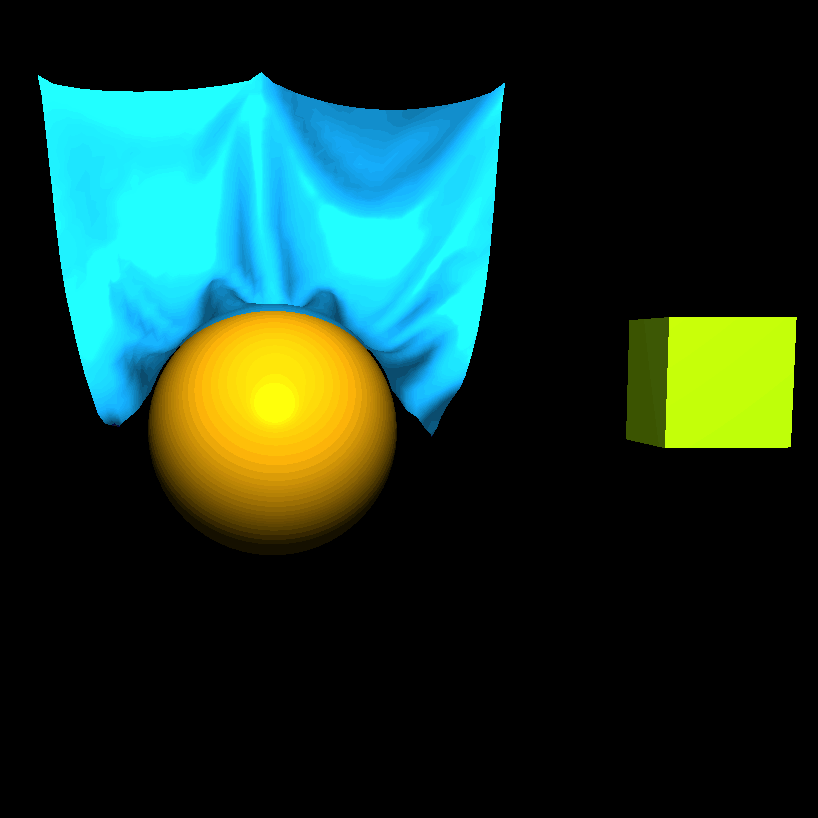
\includegraphics[width=6cm,height=6cm]{fixedMass.png}
	\caption{Draging the centre of the upper edge}
\end{figure}
\section{Results}
% pictures should be in
You can run this program as you will to see the animation, here in this report I can not present the whole performance of it.
\end{document}
